\documentclass[aspectratio=169]{beamer}
\usepackage{fancyvrb}
\usepackage{framed}
\usepackage{caption}
\usepackage{qrcode}
\usepackage{amsmath}
\usetheme{CambridgeUS}
\usepackage{hyperref}
\newcommand{\bluelink}[2]{\href{#1}{\textcolor{blue}{\textbf{#2}}}}
\usepackage{fancyvrb}

\usepackage{listings}
\usepackage{xcolor}
\usepackage{tikz}
\usetikzlibrary{shapes.geometric, arrows, positioning}

\lstdefinelanguage{smtlib}{
    keywords={declare-const, assert, check-sat, get-model},
    sensitive=true,
    morecomment=[l]{;},
    morestring=[b]",
}
\lstset{
    basicstyle=\ttfamily\small,
    keywordstyle=\color{blue},
    commentstyle=\color{gray},
    numbers=none,
    frame=single,
    captionpos=b,
    breaklines=true,
}

\tikzstyle{process}  = [rectangle, minimum width=3cm, text centered, draw=black, fill=orange!30]
\tikzstyle{decision} = [rectangle, minimum width=3cm, text centered, draw=black, fill=green!30]
\tikzstyle{code}     = [rectangle, minimum width=3cm, text centered, draw=black, fill=yellow!20]
\tikzstyle{arrow} = [thick,->,>=stealth]
\tikzstyle{arrow2} = [thick, dashed, ->,>=stealth]
\tikzstyle{arrow3} = [thick, ->, draw=blue]

\title[hevm]{
A gentle introduction to formal verification of Ethereum smart contracts}
\author[Soos]{Mate Soos}
\institute[Argot]{\large Argot Collective (\url{https://argot.org})}
\date{9th of July 2025}
\subtitle{Brussels 4th Summer School on Security Testing and Verification}

\begin{document}
\begin{frame}
    \titlepage
\end{frame}

\begin{frame}{A bit about myself}
\begin{itemize}
\item PhD from INRIA Grenoble, France
\item Part-time research at Kuldeep Meel's group, authored::
    \begin{itemize}
        \item \textbf{CryptoMiniSat} -- SAT solver with XORs
        \item \textbf{Ganak\&ApproxMC} -- CNF counters
        \item \textbf{Arjun} -- CNF simplifier
        \item \textbf{Bosphorus} -- ANF simplifier
        \item \textbf{Pepin} -- DNF counter
    \end{itemize}
\item Worked in IT Security for 10+ years: hacking,
    threat modelling, risk management
\item Working at Ethereum Foundation, now Argot Collective for the past $\approx3$
    years: \textbf{hevm}
\end{itemize}
\end{frame}

% Outline frame
\begin{frame}{Outline}
    \tableofcontents
\end{frame}

\section{Blockchain}
\begin{frame}{What is a Blockchain -- Transaction}
\begin{center}
\includegraphics[scale=0.5]{transaction}
\end{center}
\vfill
\vfill
\vfill

\tiny
Illustration from: \url{takenobu-hs/ethereum-evm-illustrated}, BSD License
\end{frame}

\begin{frame}{What is a Blockchain -- Block}
\begin{center}
\includegraphics[scale=0.5]{blockchain}
\end{center}
\vfill

\tiny
Illustration from: \url{takenobu-hs/ethereum-evm-illustrated}, BSD License
\end{frame}

\begin{frame}{What is a Blockchain -- Consensus}
\begin{center}
\includegraphics[scale=0.5]{world-state}
\end{center}
\vfill


\tiny
Illustration from: \url{takenobu-hs/ethereum-evm-illustrated}, BSD License
\end{frame}

\begin{frame}{What is a Blockchain -- Overview}
A blockchain is a \textbf{distributed ledger} that is replicated across many nodes. It is:
\begin{itemize}
    \item \textbf{Immutable} -- once written, it cannot be changed
    \item \textbf{Append-only} -- once written, it cannot be deleted
    \item \textbf{Transparent} -- anyone can see the contents of the blockchain
    \item \textbf{Decentralized} -- no single entity controls the blockchain
    \item \textbf{Consensus-based} -- nodes agree on the state of the blockchain: PoW/PoS
    \item \textbf{Permissionless} -- anyone can participate in the network (censorship resistant)
    \item \textbf{Trustless} -- no need to trust any single entity, the system works as a whole
\end{itemize}
\bigskip

Immutable caveat: except when everyone agrees it should be undone$\ldots$ (see
the DAO hack)
\end{frame}

\begin{frame}{Ethereum Blockhain}
You can think of it as a very fancy transition system that is:
\begin{itemize}
    \item \textbf{Programmable} -- it can execute code, i.e. smart contracts (via EVM)
    \item \textbf{Open-source} -- the code is available for anyone to inspect and contribute (via GitHub)
    \item \textbf{Community-driven} -- the development is driven by the community (e.g. ACD meetings)
    \item \textbf{Interoperable} -- it can interact with other blockchains and systems (via bridges)
    \item \textbf{Ever-evolving} -- it changes every ~6mo via ``hard-forks'' driven by EIPs
    \item \textbf{Scaling via L2s} -- used as a settlement layer for L2s: ZK, optimistic rollups
\end{itemize}
\bigskip

Currently, 30TPS on mainnet. Layer 2s can handle much more, but with lower guarantees.
\end{frame}

\begin{frame}{What is Ethereum used for?}

Decentralized:
\begin{itemize}
    \item \textbf{Finance} -- enables new financial systems and applications
    \item \textbf{IAM} -- enables new ways of managing identity and access management
    \item \textbf{Governance} -- enables new ways of managing and governing systems
    \item \textbf{Marketplaces} -- enables new ways of buying and selling goods and services
    \item \textbf{Gaming} -- enables new ways of playing and interacting with games
\end{itemize}
\bigskip

Some of these are simply re-packaging of existing concepts in a
in a decentralized context. Here, the \textbf{permissionless} and
\textbf{ACID} properties can sometimes come very handy.
\end{frame}

\begin{frame}{Decentralized Applications (dApps) on Ethereum}
\begin{itemize}
    \item \textbf{MakerDAO} -- stablecoin protocol
    \item \textbf{Uniswap, Suhiswap} -- exchange for trading tokens
    \item \textbf{ENS} -- domain name system for Ethereum addresses
    \item \textbf{Gitcoin} -- platform for funding open-source projects
    \item \textbf{Aave, Compund} -- lending and borrowing protocol
    \item \textbf{Tornado Cash} -- ZK-based privacy mixer for transactions
    % \item \textbf{Flashloans} -- instant loans without collateral
\end{itemize}
\end{frame}

\begin{frame}{Let's Explore}
\begin{itemize}
    \item UniSwap: \url{https://app.uniswap.org/}
    \item UniSwap Fees Collected: \bluelink{https://dune.com/gammastrategies/Uniswap-v3-Volume-and-Fees-Collected}{dashboard} Dune analytics
    \item AAVE: \url{https://app.aave.com/markets/}
    \item ENS: \url{https://app.ens.domains/}
    \item Gitcoin: \url{https://impact.gitcoin.co/}
    \item MEV: \url{https://libmev.com/}
    \item Betting: \url{https://polymarket.com/}
    \item L2s: \url{https://l2beat.com/scaling/summary}
    \item dApps: \url{https://www.growthepie.com/applications}
\end{itemize}
\end{frame}


\begin{frame}{Use-case: Flashloans}
Flashloans are a type of loan that allows you to borrow assets without
collateral, as long as you return the assets within the same transaction.
\bigskip

Remember, it's ACID, so:
\begin{itemize}
\item User asks contract for a flashloan + provides functions to call
\item Contract blindly executes the functions, with 1B+ USD in assets
\item Contract checks that the loan is repaid at the end of the transaction
\item If the loan is not repaid, the transaction is reverted
\end{itemize}
\smallskip

Can be used for:
\begin{itemize}
    \item Arbitrage -- taking advantage of price difference between exchanges
    \item Liquidation -- borrow, liquidate collateral, immediately sell, repay loan
    \item Collateral swapping -- swapping collateral in a loan
\end{itemize}
\end{frame}

\begin{frame}{Use-case: Flashloans -- Example}
Example flashloan transaction via
\bluelink{https://app.blocksec.com/explorer/tx/eth/0xe3f0d14cfb6076cabdc9057001c3fafe28767a192e88005bc37bd7d385a1116a?line=5&debugLine=5}{BlockSec Explorer}
\bigskip

Notice:
\begin{itemize}
    \item Flash loan function is \texttt{FlashLoanLogic.executeFlashLoanSimple}
    \item User-defined action is executed in the \texttt{executeOperation}
    \item Ends with \texttt{handleRepayment} which checks that the loan is repaid
    \item Notice: \texttt{transferUnderlyingTo} was ran with 47352823905004708422332 wei -- currently around 140M USD
    \item Repayment was 47376500316957210776543 wei -- difference is ~70K USD called the \texttt{premium}
\end{itemize}
\smallskip

Etherscan
\bluelink{https://etherscan.io/tx/0xe3f0d14cfb6076cabdc9057001c3fafe28767a192e88005bc37bd7d385a1116a}{view of the transaction.}
Net ``profit'' for the ``attacker'': ~7M USD
\end{frame}

\begin{frame}{Use-case: Tornado Cash}
Tornado Cash is a privacy-focused smart contract that allows users to send
ETH and ERC20 tokens anonymously. It uses zero-knowledge proofs to ensure that
the sender and receiver addresses are not linked, while still allowing the
network to verify that the transaction is valid.
\begin{itemize}
    \item Tornado Cash 0.1
        ETH \bluelink{https://etherscan.io/address/0x12d66f87a04a9e220743712ce6d9bb1b5616b8fc}{etherscan view}
    \item Example
        \bluelink{https://etherscan.io/tx/0x6d503e39f3a5cfe3736963685d7c49823a8b9de114d74331f4f44b99426cf4d5}{transaction}
    $\rightarrow$ Click ``decode input data''

\item ZK proof: verifier can check that prover knows the secret without
    revealing it
\item Think of it as RSA: you can verify that someone knows the private key
    without them revealing it.
\end{itemize}
\end{frame}

\begin{frame}{The Layers of Ethereum}
\begin{itemize}
    \item \textbf{Execution layer} -- executes the code of smart contracts as triggered by
        transactions. Performed by the EVM
    \item \textbf{Consensus layer} -- ensures all nodes agree on the state of the blockchain.
        Currently managed via proof-of-stake.
    \item \textbf{Data Availability Layer} --  ensures that transaction data is
        available (e.g. via data availability sampling)
    \item \textbf{**Application layer} -- provides the user interface and
        interaction with the blockchain (dApps)
\end{itemize}
\bigskip

The execution layer is the most important for us, as it is where the smart
contracts are executed.
\end{frame}


\section{EVM}
\begin{frame}{EVM}
    \textbf{EVM executes the code} of smart contracts and updates the state of the blockchain:
\begin{itemize}
    \item Stack machine -- instead of registers, it uses a stack
    \item Everything is 256b by default, addresses are 160b
    \item No undefined behaviour
    \item No IO. No printing, disk, networking, etc.
    \item Only has a few regions for data: returndata, calldata, memory, storage, (stack)
    \item No pointers. One contiguous memory, calldata, and returndata region
    \item No such thing as infinite loops: gas is a unit of execution that is always limited
    \item No such thing as huge memory/storage usage: gas also limits memory and storage
    \item Can call other contracts, allowing for composability
    \item ACID-compliant -- provides atomicity, consistency, isolation, and durability
\end{itemize}
\smallskip

Note: \textbf{Solana uses eBPF}, which was mentioned during the static code analysis seminar
\end{frame}

\begin{frame}{EVM Overview}
\begin{center}
    \includegraphics[scale=0.5]{EVM-state}
\end{center}
\vfill

\tiny
Illustration from: \url{takenobu-hs/ethereum-evm-illustrated}, BSD License
\end{frame}

\begin{frame}{EVM Instructions Overview}
The EVM has a set of instructions that can be used to manipulate the state of the
blockchain.
\smallskip

Instruction categories:
\begin{itemize}
    \item \textbf{Arithmetic/Logic Ops} -- basic operations like add, multiplication, div, $\ldots$
    \item \textbf{Control Flow Ops} -- jumps, program counter, halting, revert, $\ldots$
    \item \textbf{Stack/Memory/Storage Ops} -- stack manipulation, memory\&storage access, $\ldots$
    \item \textbf{External Calls and Contracts} -- calling contracts, transferring value, creating contracts
    \item \textbf{Context Ops} -- accessing block context, gas information, contract information, logging
\end{itemize}
\bigskip

Let's check out \url{https://www.evm.codes/}
\bigskip

Let's try 8/8 and then 2/0 (i.e. division by zero), in the \bluelink{https://www.evm.codes/playground}{EVM Playground}.

Load in Bytecode: \texttt{60086008046002600004}
\end{frame}

\begin{frame}{EVM vs x86 ADD}
EVM \bluelink{https://www.evm.codes/}{add instruction}:
\begin{itemize}
    \item Takes two numbers from the stack, adds them mod $2^{256}$, pushes the
        result to the stack
    \item If it runs out of gas, reverts the frame
\end{itemize}
\bigskip
The OF, SF, ZF, AF, CF, and PF flags are set according to the result.
x86 \bluelink{https://www.felixcloutier.com/x86/add}{add instruction}:
\begin{itemize}
    \item Depending on the variation of the opcode, it'll add different registers together
    \item Depending on the variation of the opcode, it will add them over different bit sizes
    \item The OF, SF, ZF, AF, CF, and PF flags are set according to the result
    \item It might throw an exception
\end{itemize}
\bigskip

Q: Which one is easier to reason about?
\end{frame}

\begin{frame}{EVM Instructions Part 1}

\begin{block}{Arithmetic/Logic (ALU) Operations}
\begin{itemize}
    \item Basic arithmetic: \texttt{ADD}, \texttt{SUB}, \texttt{MUL}, \texttt{DIV}, \texttt{MOD}, \texttt{EXP}, \texttt{SIGNEXTEND}
    \item Bitwise operations: \texttt{AND}, \texttt{OR}, \texttt{XOR}, \texttt{NOT}
    \item Comparisons: \texttt{LT}, \texttt{GT}, \texttt{EQ}, \texttt{ISZERO}, \texttt{SLT}, \texttt{SGT}
    \item Shift operations: \texttt{SHL}, \texttt{SHR}, \texttt{SAR}
    \item Special operations: \texttt{KECCAK256}
\end{itemize}
\end{block}

\begin{block}{Control Flow Operations}
\begin{itemize}
    \item Jumps: \texttt{JUMP}, \texttt{JUMPI}
    \item Program counter: \texttt{PC}
    \item Halting: \texttt{STOP}, \texttt{RETURN}, \texttt{REVERT}
\end{itemize}
\end{block}
\end{frame}

\begin{frame}{Control Flow, Code and Data Separation}
\begin{itemize}
    \item You can only jump to already deployed code -- no dynamic code generation
    \item Code points that can be jumped to are marked with \texttt{JUMPDEST}
    \item Code is immutable, but we can \texttt{JUMP/JUMPI} to a dynamically
        computed position
    \item So computing a Control Flow Graph (CFG) can be hard/impossible
    \item It's possible to jump into the middle of a PUSH instruction,
        if the PUSH-ed data happens to match the JUMPDEST opcode
    \item So it's data and code separation is not as clear-cut
\end{itemize}
\end{frame}

\begin{frame}{EVM Instructions Part 2}
\begin{block}{Stack/Memory/Storage Operations}
\begin{itemize}
    \item Stack manipulation: \texttt{PUSH}, \texttt{POP}, \texttt{DUP}, \texttt{SWAP}
    \item Memory access: \texttt{MLOAD}, \texttt{MSTORE}
    \item Storage: \texttt{SLOAD}, \texttt{SSTORE}, \texttt{TSLOAD}, \texttt{TSSTORE}
    \item Calldata: \texttt{CALLDATALOAD}, \texttt{CALLDATASIZE}, \texttt{CALLDATACOPY}
    \item Return data: \texttt{RETURNDATASIZE}, \texttt{RETURNDATACOPY}
    \item Code access: \texttt{CODECOPY}, \texttt{EXTCODECOPY}
\end{itemize}
\end{block}


\begin{block}{External Calls and Contracts}
\begin{itemize}
    \item Call ops: \texttt{CALL}, \texttt{CALLCODE}, \texttt{DELEGATECALL}, \texttt{STATICCALL}
    \item Value transfer: \texttt{CALLVALUE}, \texttt{TRANSFER}
    \item Contract creation: \texttt{CREATE}, \texttt{CREATE2}, \texttt{SELFDESTRUCT}
\end{itemize}
\end{block}
\end{frame}

\begin{frame}{EVM Instructions Part 3}
\begin{block}{Context}
\begin{itemize}
    \item Block Context: \texttt{COINBASE}, \texttt{TIMESTAMP}, \texttt{NUMBER},
        \texttt{PREVRANDAO},
        \texttt{ADDRESS}, \texttt{BALANCE}, \texttt{ORIGIN},  \texttt{CALLER},
        \texttt{BLOCKHASH}, \texttt{DIFFICULTY}, \texttt{BLOBHASH},
        \texttt{BLOBBASEFEE}, \texttt{CHAINID}
    \item Gas: \texttt{GAS}, \texttt{GASLIMIT}, \texttt{GASPRICE}
    \item Contract information: \texttt{EXTCODESIZE}, \texttt{EXTCODEHASH},
        \texttt{MSIZE}
    \item Logging: \texttt{LOG}
\end{itemize}
\end{block}
\end{frame}


\begin{frame}{ABI}
The Application Binary Interface (ABI) is the interface between smart contracts
and external applications. It defines how to encode and decode data for
function calls, events, and errors.
\bigskip

The ABI is used to:
\begin{itemize}
    \item Encode function calls and parameters
    \item Decode return values
    \item Handle errors
\end{itemize}
\end{frame}

\begin{frame}[fragile=singleslide]{ABI function call}
\begin{itemize}
    \item Function signature is a 4-byte hash of the function name and its parameter types
    \item Function parameters follow, with packed encoding (e.g. 4 uint64-s will be packed into 32 bytes)
\end{itemize}
\bigskip

Example:
\begin{Verbatim}[frame=single, framerule=0.2mm, framesep=2mm,fontsize=\small]
$ cast keccak "get()"
0x6d4ce63caa65600744ac797760560da39ebd16e8240936b51f53368ef9e0e01f
\end{Verbatim}
Hence, the function signature for \texttt{get()} is \texttt{0x6d4ce63c}. So:

\begin{Verbatim}[frame=single, framerule=0.2mm, framesep=2mm,fontsize=\small]
(bool success, bytes memory data) = address(myContract).call("get()");
\end{Verbatim}

will generate the calldata \texttt{0x6d4ce63c} as the first 4 bytes, followed by 0 bytes for the empty parameters.
\end{frame}

\begin{frame}[fragile=singleslide]{ABI error/panic}
\begin{Verbatim}[frame=single, framerule=0.2mm, framesep=2mm,fontsize=\small]
(bool success, bytes memory data) = address(myContract).call(
    abi.encodeWithSignature("myfun(uint256)", 42));
if (!success) {
    bytes4 errorSelector;
    assembly { errorSelector := mload(add(data, 0x20)) }
    if (errorSelector == bytes4(keccak256("Error(string)"))) {
        string memory reason = abi.decode(data, (string));
        // reason is a string, e.g. "revert"
    } else if (errorSelector == bytes4(keccak256("Panic(uint256)"))) {
        uint256 code = abi.decode(data, (uint256));
        // Panic code is a uint256, e.g. 0x11
    }
}
\end{Verbatim}
\end{frame}

\begin{frame}{EVM: Panic Codes}
\begin{itemize}
    \item 0x00: Generic compiler inserted panics.
    \item 0x01: Call assert with an argument that evaluates to false.
    \item 0x11: Arithmetic operation results in underflow or overflow
    \item 0x12; Divide or modulo by zero (e.g. 5 / 0 or 23 \% 0).
    \item 0x21: Convert a value that is too big or negative into an enum type.
    \item 0x22: Access a storage byte array that is incorrectly encoded.
    \item 0x31: Call .pop() on an empty array.
    \item 0x32: Access an array, bytesN or an array slice at an out-of-bounds
        or negative index (i.e. $x[i]$ where $i >= x.length$ or $i < 0$).
    \item 0x41: Allocate too much memory or create an array that is too large.
    \item 0x51: Call a zero-initialized variable of internal function type.
\end{itemize}
\end{frame}


\begin{frame}{Programming the EVM}
We use Solidity to program the EVM, with YUL inline assembly: \begin{itemize}
    \item \textbf{Imperative}, high-level language -– Code is executed
        step-by-step (like C++). \item \textbf{Statically typed} -- Variable
        types must be declared at compile time (e.g., uint, string). \item
        \textbf{Object-oriented} -- Supports contracts ($\approx$classes),
        inheritance, interfaces, and libraries. \item \textbf{Smart contract
        focus} -- Designed for writing decentralized apps (dApps) \item
        \textbf{Special features} -- Built-in globals (e.g., msg.sender), ABI
        en\&decoding
\end{itemize}
\bigskip

\url{https://docs.soliditylang.org/en/v0.8.30/}
\end{frame}

\begin{frame}{Solidity vs EVM bytecode}
\begin{itemize}
    \item Solidity is a high-level language that compiles to EVM bytecode
    \item Provides a more readable and maintainable way to write contracts
    \item EVM bytecode is what is actually executed by the EVM
    \item The two are \textbf{connected} via a hash that's added at the end of the bytecode
    \item Hash, along with the contract code can be submitted to e.g. sourcify.eth
    \item Click on  \bluelink{https://sourcify.dev/}{sourcify.eth} and look up
        \texttt{0x1F98431c8aD98523631AE4a59f267346ea31F984} -- the UniSwapv3 contract
    \item Click \texttt{View in Sourcify Repository} to see the source code
\end{itemize}
\end{frame}

\begin{frame}{Online development environment: Remix}
Built-in:
\begin{itemize}
    \item Solidity compiler
    \item Test deployment environment
    \item Debugger
    \item Unit testing
    \item GitHub integration
\end{itemize}
\bigskip

\bluelink{https://remix.ethereum.org/}{Remix Online IDE}:
Load a \bluelink{https://github.com/msooseth/remix-example}{simple Remix GitHub project}

Check tests: \texttt{a.complicated(10,9)} could be made to fail.
\end{frame}


\begin{frame}[fragile=singleslide]{Solidity: Special Functions: constructor,
    receive, fallback}
You can define special functions in Solidity that will be called when
the contract is \textbf{created},
when the contract \textbf{receives Ether} without a function call,
or when a \textbf{function is not found},

\begin{Verbatim}[frame=single, framerule=0.2mm, framesep=2mm,fontsize=\small]
interface RemoteContract {
    function withdraw() external;
}
contract Attacker{
    RemoteContract remote;
    uint receives = 0;
    uint fallbacks = 0;

    constructor(address addr) { remote = RemoteContract(addr); }
    receive() external payable { receives++; }
    fallback() external { fallbacks++; }
}
\end{Verbatim}
\end{frame}

\begin{frame}{Solidity: Special Functions: constructor, receive, fallback --
    part 2}
Who sees the issues with this?
\pause
\bigskip

\textbf{Can't just send Ether to the contract, it might take control of execution}
\begin{itemize}
    \item It might call us back! Reentrancy attack.
    \item It might call other contracts we rely on, changing their state
    \item It might manipulate the cost of some asset whose price we already
        calculated/saved
\end{itemize}
\bigskip

All calls\&transfers to external contracts require \textbf{careful
consideration}.
\end{frame}

\begin{frame}{The DAO Hack}
The DAO hack (in 2016) was a major event in Ethereum's history, where an
attacker exploited a \textbf{reentrancy vulnerability} in the DAO contract to
steal \$50 million worth of Ether.

The hack led to a hard fork of Ethereum, creating Ethereum
Classic (ETC) and Ethereum (ETH).
\end{frame}

\begin{frame}{The DAO Hack -- Let's do it!}
Let's recreate the DAO hack in Remix!
\begin{enumerate}
\item    Load
    \bluelink{https://github.com/msooseth/reentrancy-attack-challenge}{this
    GitHub repo} into Remix
\item    Compile \& Deploy \textbf{FundRaiser}
\item    Compile \& Deploy \textbf{Attacker}, with \textbf{FundRaiser} address
    as parameter
\item    Set \textbf{Value} to 10000 and call \textbf{deposit} on Fundraiser.
    This will deposit money on YOUR balance
\item    Call \textbf{getTotalFunds} on Fundraiser. Should show 10000.
\item    Set \textbf{Value} to 400 and call \textbf{depositFunds} on Attacker.
    This will deposit money on the ATTACKER's balance
\item    Call \textbf{getTotalFunds} on Fundraiser. Should show 10400.
\item    Call \textbf{getFunds} on Attacker. Should show 0. The attacker has 0
    funds currently.
\item    Call \textbf{withdrawFunds} on Attacker. This is the attack.
\item    Call \textbf{getFunds} on Attacker. Should show 1600 -- 4x what the
    Attacker deposited!
\end{enumerate}
\end{frame}

\begin{frame}{Example: Tornado Cash's Reentrancy Guard}
Uses a decorator
\bluelink{https://github.com/tornadocash/tornado-core/blob/master/contracts/Tornado.sol}{ReentracyGuard}
to prevent reentrancy attacks:
\bigskip

The actual implementation of the guard is by
\bluelink{https://github.com/OpenZeppelin/openzeppelin-contracts/blob/master/contracts/utils/ReentrancyGuard.sol}{openzeppelin}
\bigskip

Simple solution: \texttt{\_status} variable set to 1/2 depending on whether
we have entered the function or not. If we try to enter the function again, we
fail the \texttt{\_status == ENTERED} check, and revert the transaction.
\end{frame}


\section{Testing and Verification}
\begin{frame}{What is a bug anyway?}
EVM:
\begin{itemize}
    \item Steal the money due to e.g. overflow/reentrancy/logical error/etc bug
    \item Lock in the money due to liveness issues
    \item Exploit incorrect rounding in online exchanges to drain contract
    \item Borrow money to buy some asset, dump it in an automated market maker
        pushing its price to zero, then buy everything for zero.
\end{itemize}

Consensus:
\begin{itemize}
    \item \bluelink{https://arxiv.org/pdf/1904.05234}{Frontrunning}:
        observe a money-making transaction, replace the
        recipient of the transaction with my own address
    \item \bluelink{https://etherscan.io/tx/0xee9fcd2b9996e96b642cb4cda47fc140f98fdaf07ee02657743d4bfcc4670106}{Sandwiching}:
        see someone is buying an asset, buy a lot of
    the asset before their transaction is executed, then sell it all off
    later for a higher price. Block is
    \bluelink{https://etherscan.io/txs?block=22029771}{here}, observe the \texttt{MEV Bot}
    before and after the \texttt{0xee9fc} transaction.
    (\bluelink{https://x.com/nikokampouris/status/1899914224484147661}{X
    thread}, \bluelink{https://zeromev.org/block?num=13640275}{another} example)
\end{itemize}

\bigskip
Some of these are ''clearly`` bugs. Some of them are abuse of
systems(frontrunning). Some are games played according to the rules, but
perhaps not according to the spirit.
\end{frame}

\begin{frame}{The Testing Pyramid}
\centering
\includegraphics[scale=0.8]{triangle3}
\end{frame}


\begin{frame}{The Testing Continued}
\begin{itemize}
    \item Things get more expensive as you go up the pyramid
    \item Test types
    \begin{itemize}
        \item Positive test: correct password -- should log in
        \item Negative test: incorrect password -- should not log in
        \item Invariant test: total balance of all accounts should not change
    \end{itemize}
    \item Exploratory testing:
    \begin{itemize}
        \item manual review: auditing by a human
        \item fuzz testing: ``randomly'' generate inputs to find bugs
        \item symbolic execution: compute all possible inputs to find bugs
    \end{itemize}
\end{itemize}
\end{frame}

\begin{frame}{Fuzzing}
You just had a long lecture so I won't go into details :)
Tools in Ethereum:
\begin{itemize}
    \item \textbf{Echidna}: Coverage-guided fuzzer for Ethereum smart
        contracts, via \textbf{hevm}
    \item \textbf{Forge}: Built-in fauzzer as part of Foundry, only recently
        coverage-guided, via \textbf{reth}
    \item \textbf{Medusa}: Fuzzer for Ethereum smart contracts via fork of
        \textbf{geth}
\end{itemize}
\bigskip

Why specialized execution engines? Because we need:
\begin{itemize}
    \item \textbf{Cheat Codes} -- special functions to
        \bluelink{https://getfoundry.sh/reference/cheatcodes/environment}{manipulate the world state}
    \begin{itemize}
        \item \textbf{deal} -- gives ETH to an address
        \item \textbf{prank} -- changes the sender of the transaction
        \item \textbf{roll} -- changes the block number
        \item \textbf{...}
    \end{itemize}
    \item \textbf{Coverage Metrics} -- we need to know which parts of the code
        were executed
\end{itemize}
\end{frame}

\section{Symbolic Execution}
\begin{frame}[fragile=singleslide]{Symbolic Execution vs Fuzzing}
Say your code is:

\begin{Verbatim}[frame=single, framerule=0.2mm, framesep=2mm,fontsize=\small]
function tricky(uint a, uint b) public pure {
	// solution: a = 10000983843024
	//           b = 9877982748934

	if (a * 2 + b == 29879950434982 &&
	    b / 2 == 4938991374467) {
		assert(false); // bad things happen
	}
}
\end{Verbatim}
Fuzzing never finds this edge-case. Symbolic execution always finds it.
\bigskip

\textbf{In general, fuzzing is faster, but is incomplete. Symbolic execution is
slower but complete.}
\end{frame}

\begin{frame}[fragile=singleslide]{Symbolic Execution: straight line program}
Most execution works by running instructions concretely:
\begin{verbatim}
---             ax: 1   , bx: 2
mov %bx %ax     ax: 2   , bx: 2
add %ax $4      ax: 6   , bx: 2
\end{verbatim}
\bigskip

Symbolic execution, with symbolic state:
\begin{verbatim}
---             ax: v1  , bx: v2
mov %bx %ax     ax: v2  , bx: v2
add %ax $4      ax: v2+4, bx: v2
\end{verbatim}
\end{frame}

\begin{frame}[fragile=singleslide]{Symbolic Execution -- branching}
\begin{minipage}[t]{0.45\textwidth}
Concrete execution:
\begin{Verbatim}[fontsize=\small]
-----------     ax: 1    bx: 1
cmp %ax %bx     ax: 1    bx: 1
je .if_true
; false
add %ax $4
jmp short .end
.if_true:
add %ax $5      ax: 6    bx: 1
.end:
\end{Verbatim}
\end{minipage}%
\begin{minipage}[t]{0.45\textwidth}
Symbolic execution, with symbolic state:
\begin{Verbatim}[fontsize=\small]
-----------     ax: v1   bx: v2
cmp %ax %bx
je .if_true
; false
add %ax $4      ax: v1+4 bx: v2
jmp short .end
.if_true:
add %ax $5      ax: v1+5 bx: v2
.end:
\end{Verbatim}
\begin{Verbatim}[fontsize=\small]
-**- v1==v2 ->  ax: v1+5 bx: v2
-**- v1!=v2 ->  ax: v1+4 bx: v2
\end{Verbatim}
\end{minipage}
\bigskip

For symbolic execution, we end up having to follow two executions. This can become exponential.
\end{frame}

\begin{frame}{Path Explosion}
\bluelink{https://github.com/ethereum/hevm/issues/763}{hevm struggling}
with path explosion
\smallskip

Potential solutions:
\begin{itemize}
    \item \textbf{Path pruning} -- dispatch partial path conditions, stop
        exploring paths that are already known to be infeasible
    \item \textbf{Path merging} -- merge paths that have the same state
    \item \textbf{Lookahead} -- check if any assert failure is reachable
        from this path at all
\end{itemize}
\smallskip

Just some insight:
\bluelink{https://github.com/a16z/halmos/issues/346}{halmos'
todo list}
\end{frame}

\begin{frame}{Related Work}
Symbolic execution is used in two major ways. One is to \textbf{validate static
code analysis} results, the other is \textbf{pure symbolic execution}. The
first approach is followed by Oyente, sCompile, Mythril, etc. These are
typically incomplete, and false positives are allowed.

\bigskip

Purely symbolic execution-based systems:
\begin{itemize}
\item \textbf{halmos}: Written in python, with its own IR and internal rewrite
    engine
\item \textbf{Certora Prover}: Based on backwards exploration and weakest
    precondition computation, uses CVL specification language
\item \textbf{KEVM}: K-framework based, allows to ``break out'' into K to prove lemmas
\item \textbf{EthBMC}: Bounded model checking-based exploration of contracts
\end{itemize}
\end{frame}

\section{hevm -- EVM Symbolic Execution}
\begin{frame}{Overview of hevm}
\begin{itemize}
\item Started $\approx7$ years ago as part of dapptools, but is now a standalone tool
\item Implements EVM semantics for concrete and symbolic execution
\item Examines \emph{all}\footnote{loops/recursion is an issue, we have a loop/depth limit} execution paths from the starting state
\item Finds the set of requirements to reach all failing paths
\item Runs external SMT solver(s) to find input to reach them
\item Displays call needed to trigger fault/discrepancy
\end{itemize}
\end{frame}

\begin{frame} {Satisfiability Modulo Theories (SMT) Solvers}
\textbf{What is an SMT solver?}
\begin{itemize}
    \item Extends SAT solvers by supporting \textbf{first-order logic with theories} (e.g., arithmetic, arrays, bit-vectors)
    \item Decides the satisfiability of logical formulas over \textbf{background theories}
\end{itemize}

\textbf{Key Applications:}
\begin{itemize}
    \item Formal verification (hardware/software)
    \item Program analysis (symbolic execution)
    \item Automated theorem proving
\end{itemize}

\textbf{Example Theory Combinations:}
\begin{itemize}
    \item Bit-vectors: $x \ll 2 == 0b1000$
    \item Arrays: $A[i] = A[j]$
    \item Uninterpreted functions: $f(x) = f(y)$
\end{itemize}
\end{frame}

\begin{frame}[fragile=singleslide]{SMT Solving in Practice}
\textbf{Example Query (Using Z3 Syntax):}
\begin{lstlisting}[language=smtlib]
(declare-const x Int)
(declare-const y Int)
(assert (>= x 0))
(assert (>= y 0))
(assert (= (+ (* 2 x) y) 10))
(check-sat)
(get-model)
\end{lstlisting}
\textbf{Result:}
Solver finds a satisfying model, e.g., $x = 5$, $y = 0$
\bigskip

\textbf{Why SMT?}
\begin{itemize}
    \item Combines \textbf{SAT} efficiency with \textbf{domain-specific reasoning}
    \item Theories to model: bitvectors, arrays, arithmetic, and
        uninterpreted functions (AUFBV)
\end{itemize}
\end{frame}

\begin{frame}[fragile=singleslide]{SMT solver hands-on: z3 in the browser}
You can play with \bluelink{https://jfmc.github.io/z3-play/}{z3 in your browser}
\bigskip

Example bitvector query:
\begin{lstlisting}[language=smtlib]
(set-logic QF_BV)
(declare-const x (_ BitVec 8))
(declare-const y (_ BitVec 8))
(assert (= (bvadd x y) (_ bv7 8)))
(check-sat)
(get-model)
\end{lstlisting}
\bigskip

Let's require that one is $>7$:
\begin{lstlisting}[language=smtlib]
(assert (bvugt x (_ bv7 8)))
\end{lstlisting}
\end{frame}

\begin{frame}{hevm: How to define what's a bug?}
\begin{itemize}
    \item We decided NOT to enforce any ``opinions'' on what a bug is
    \item We don't have a specification language, unlike e.g. Certora Prover's CVL
    \item The spec has to be expressed in-line code via require/assert
    \item If used as a library, interface exists to specify pre/post-conditions
\end{itemize}

\bigskip
This way we allow others to be opinionated, but we ourselves remain unopinionated.

But: it misses the ability to express some invariants, e.g. ``total balance of
all accounts should not change''.
\end{frame}

\begin{frame}{Certora Verification Language (CVL)}
Certora Prover uses a specification language called CVL to express properties
of the contract. CVL is a domain-specific language for writing specifications
of smart contracts. It allows you to express properties of the contract in a
declarative way, and then prove that the contract satisfies these properties.

\bigskip

Example
\bluelink{https://github.com/Certora/tutorials-code/tree/master/lesson4_invariants/sqrt}{CVL
specification} for SQRT approximation over fixed-point numbers.
\end{frame}

\begin{frame}[fragile=singleslide]{Symbolic Execution: Example}
Say your code looks like this:
\begin{Verbatim}[frame=single, framerule=0.2mm, framesep=2mm,fontsize=\small]
function overflow(uint a) public pure {
  uint b;
  unchecked { b = a + 1;}
  assert(b > a);
}
\end{Verbatim}

hevm can find the case where $a=0xffffff\ldots$ to trigger the assert due to
roll-around. hevm gives you the \textbf{exact call to reproduce the bug}. This
way of using hevm can find a \emph{known-bad state}.
\end{frame}

\begin{frame}[fragile=singleslide]{Symbolic Execution: Invariant Checking}
You can describe \textbf{invariants} of your contract and write them as
functions Then assert these functions every time the invariant must hold.
\begin{Verbatim}[frame=single, framerule=0.2mm, framesep=2mm,fontsize=\small]
function my_invariant() private pure returns inv {
	inv = ...calculate invariant...
}

function transfer(uint a) public pure {
	require(my_invariant());
	... your function code here ....
	assert(my_invariant());
}
\end{Verbatim}

Here, instead of a known-bad state, we validate that we are always in state
that matches our expectations.
\end{frame}

\begin{frame}{hevm: Symbolic Execution for Counterexample Generation}
\centering
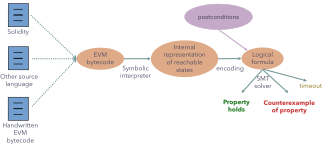
\includegraphics[scale=0.45]{pipeline}
\end{frame}

\begin{frame}{hevm: Symbolic Execution for Equivalence Checking}
\centering
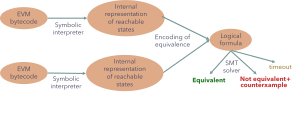
\includegraphics[scale=0.45]{equivalence-pipeline}
\end{frame}
%
%
\begin{frame}[fragile=singleslide]{hevm: Symbolic Execution for Equivalence Checking}
You can ask hevm to check whether two implementations are equivalent
\bigskip
\\

\begin{minipage}[b]{0.45\textwidth}
\begin{Verbatim}[frame=single, framerule=0.2mm, framesep=2mm,fontsize=\small]
function (...) public returns x {
  x = //known good computation
      //uses lots of gas
}
    \end{Verbatim}
  \end{minipage}
  \begin{minipage}[b]{0.45\textwidth}
  \begin{Verbatim}[frame=single, framerule=0.2mm, framesep=2mm,fontsize=\small]
function (...) public returns x {
  x = //complicated computation
      //uses less gas/
}
\end{Verbatim}
\end{minipage}

hevm can give the exact \textbf{call to trigger the discrepancy} between the two functions. This way, you can safely improve the gas performance of your code.
\end{frame}

\begin{frame}{hevm's Symbolic Executor}
hevm's symbolic executor is very powerful:
\begin{itemize}
\item \textbf{Operates on bytecode} so runs everything deployed to the chain
\item Understands \textbf{all of EVM}: stack, call frames, memory, storage, calldata
\item Can run on \textbf{any point in blockchain history} via RPC to an archive node
\item Pull all required contracts from the chain via RPC to a full node
\item Overapproximates unknown code
\end{itemize}
\bigskip

Limitations:
\begin{itemize}
\item Cannot deal with \textbf{symbolic gas} other than ignoring it
\item \textbf{Symbolic offset/size memcopy} is not implemented, but is often unneeded
\item \textbf{Loops and recursion} are explored only to a fixed depth
\end{itemize}
\end{frame}

\begin{frame}{Under- and Overapproximation}
Underapproximation:
\begin{itemize}
    \item We may \textbf{miss a counterexample} that is reachable in the
        contract.
    \item Example: \texttt{CALL} to unknown code gives up exploration,
        \textbf{prints warning}
    \item This would be a \textbf{soundness} issue, hence we \textbf{always
        warn}
\end{itemize}
\bigskip

Overapproximation:
\begin{itemize}
    \item We may return a counterexample that is \textbf{not
        actually reachable} in the contract.
    \item Example: \texttt{STATICCALL} to unknown code returns a
        fresh buffer and return value.
    \item \texttt{STATICCALL} cannot change state, so this is a valid
        overapproximation.
    \item Note: computing an \textbf{invariant of a loop} using CHC would also be
        an overapproximation
\end{itemize}
\end{frame}

\begin{frame}{hevm internals}
\centering
\includegraphics[scale=0.6]{hevm-overview}
\end{frame}


\begin{frame}[fragile=singleslide]{Intermediate Representation: Code to Expression}
\small
Through the symbolic execution engine we create an expression that captures all
end-states. We then take each end-state out and filter it for things we are
looking for, e.g. assertion failures. Let's take the example:

\begin{Verbatim}[frame=single, framerule=0.2mm,framesep=2mm,fontsize=\small]
function overflow(uint a) public pure {
    uint b;
    unchecked { b = a + 1;}
    assert(b > a);
}
\end{Verbatim}

The expression to generate a counterexamle for this could look like:
\begin{Verbatim}[frame=single, framerule=0.2mm, framesep=2mm,fontsize=\small]
PLEq (Add (Var "a") (Lit 1)) (Var "a")
\end{Verbatim}

Notice: we use less-or-equal, because we want a \textbf{counterexample}
\end{frame}

\begin{frame}[fragile=singleslide]{Intermediate Representation: Graph of Expressions}
\centering
\includegraphics[scale=0.85]{IR}
\end{frame}

 \begin{frame}[fragile=singleslide]{Intermediate Representation: Writes}
 Writing in a buffer is represented as a chain of writes:
 \begin{Verbatim}[frame=single, framerule=0.2mm, framesep=2mm,fontsize=\small]
 AbstractBuf "a" // empty buffer
 WriteWord (Lit 1) (Var "a") (AbstractBuf "a") //1st write
 WriteWord (Lit 2) (Var "b") (WriteWord (Lit 1) (Var "a") (AbstractBuf "a")) //2nd
 \end{Verbatim}

 This can later be collapsed, e.g. in case the variables are concertized. We use \texttt{(AbstractBuf "var")} for symbolic, and \texttt{(ConcreteBuf "value")} for concrete values.
 \bigskip

 Allows us to simply prepend an operation for each instruction.

 We later collapse \& simplify these writes.
 \end{frame}

 \begin{frame}[fragile=singleslide]{Intermediate Representation: Keccak}
 Keccak, i.e. SHA-3 is used extensively by all contracts. This is because \textbf{storage of contracts is an unstructured array} of uint256. Hence, to implement e.g. maps and an arrays, one needs to use Keccak to map to a "random" position in storage, so as not to clash.
 \bigskip

 It's very expensive to accurately represent Keccak in SMT. Hence, we represent Keccak as an \textbf{uninterpreted function} in SMT, with the following rules:
 \begin{itemize}
 \item We know the concrete value of the input $\rightarrow$ we add the axiom $keccak(input)=output$
 \item Size of input differs $\rightarrow$ hash differs. We assert this for all pairs
 \item Assert all pairs of keccak to be unequal if they don't match over \emph{partial} concrete values
 \item $keccak(x) > 128$. Small slot values are used for non-map/array elements of contracts
 \end{itemize}
 \end{frame}

 \begin{frame}[fragile=singleslide]{Intermediate Representation: Maps}
 Storage of contracts is an unstructured array of uint256. Solidity uses:
 $keccak (bytes32(key) || bytes32(id))$ to map $mymap[key]$ where $id$ is the
 map index:

 \begin{Verbatim}[frame=single, framerule=0.2mm, framesep=2mm,fontsize=\small]
 contract C {
     mapping(uint => uint) map_id_0;
     mapping(uint => uint) map_id_1;
 }
 \end{Verbatim}
 We have Solidity-specific rewrite rules to strip writes. So when writing two $keccak (bytes32(key) || bytes32(id))$-s on top of each other, and then reading, we traverse the list of writes to pick out the potentially matching one(s).
 \bigskip

 Notice that the SMT solver can use our Keccak rules to do this, too, but it's a lot slower
 \end{frame}

% DEVCON maybe add?
 \begin{frame}[fragile=singleslide]{Intermediate Representation: Simplification}
 We do all the following rewrites to fixedpoint:
 \begin{itemize}
     \item Constant folding
     \item Canonicalization of all commutative operators (concrete value first)
     \item Canonicalization of all less-than/greater-than/etc operators
     \item Canonicalization of all Keccak expressions to match Solidity patterns
     \item Stripping writes when they are not read
     \item Stripping reads when they are not used
     \item (In)equality propagation
     \item All meaningful rewrites, such as min/max/add+sub/add+add/sub+sub/etc.
     \item Special rewrite rules for array/map lookups and other Solidity patterns
 \end{itemize}
 \end{frame}

\begin{frame}[fragile=singleslide]{Intermediate Representation: Haskell to the Rescue}
Haskell supports algebraic data types (ADTs), so our intermediate representation (IR) can be fully typed. Furthermore, Haskell supports pattern matching, so our rewrite rules are easy to read \& write:
\begin{Verbatim}[frame=single, framerule=0.2mm, framesep=2mm,fontsize=\small]
    -- syntactic Eq reduction
    go (Eq (Lit a) (Lit b))
      | a == b = Lit 1
      | otherwise = Lit 0
    go (Eq (Lit 0) (Sub a b)) = eq a b
    go (Eq a b)
      | a == b = Lit 1
      | otherwise = eq a b
\end{Verbatim}
\end{frame}

\begin{frame}[fragile=singleslide]{What can we use the IR for?}
\begin{itemize}
    \item Finding counterexamples with SMT solvers
    \item Constant extraction: helping other fuzzers with "magic numbers"
    \item Substitute constants and fold: we can build a fuzzer
    \item Not just failing branches: automated test-case generation
    \item Review by humans: the IR is a clean representation of the problem
\end{itemize}
\end{frame}

\begin{frame}[fragile=singleslide]{Solving the IR: Creating a Fuzzer}
Fuzzing sounds strange given that hevm is a symbolic execution engine. However:
\begin{itemize}
\item The IR is actually a very clean representation of the problem at hand
\item Due to the extensive simplifications applied, it can contain specific constants that may be very hard to find otherwise
\item IR \emph{could} be transpiled to assembly (potentially through \texttt{C}), and executed as a program
\end{itemize}
\bigskip

Notice that geth, the normal EVM concrete executor is incredibly slow. Hence a transpiled IR could achieve serious speedup.
\end{frame}

\begin{frame}[fragile=singleslide]{Solving the IR: using an SMT Solver}
The IR is translated in a straightforward manner to SMT. Let's say the expression is:

\begin{Verbatim}[frame=single, framerule=0.2mm, framesep=2mm,fontsize=\footnotesize]
PLEq (Add (Var "a") (Lit 1)) (Var "a")
\end{Verbatim}

The SMT expression for this could be:
\begin{lstlisting}[language=smtlib]
(set-logic QF_AUFBV)
(define-sort Word () (_ BitVec 256))
(declare-const varA (Word))
(assert (bvule (bvadd varA (_ bv1 256)) varA))
(check-sat)
(get-model)
\end{lstlisting}

Z3 gives the answer:
\begin{Verbatim}[frame=single, framerule=0.2mm, framesep=2mm,fontsize=\footnotesize]
sat
define-fun varA () (_ BitVec 256)
    #xffffffffffffffffffffffffffffffffffffffffffffffffffffffffffffffff)
\end{Verbatim}
\end{frame}

\begin{frame}[fragile=singleslide]{Example Solidity Test}
\begin{Verbatim}[frame=single, framerule=0.2mm, framesep=2mm,fontsize=\footnotesize]
import {Test} from "forge-std/Test.sol";
contract MyContractOverflow is Test {
  uint balance = 100;
  function prove_overflow(uint amt) public {
    unchecked { balance += amt; }
    assert(balance >= amt);
  } }
\end{Verbatim}


\begin{Verbatim}[frame=single, framerule=0.2mm, framesep=2mm,fontsize=\footnotesize]
Checking 1 function(s) in contract src/overflow-test.sol:MyContractOverflow
[RUNNING] prove_overflow(uint256)
   Exploring call prefix 0x7a400a2b
   Exploration finished, 3 branch(es) to check in call prefix 0x7a400a2b
   SMT result: Cex SMTCex {vars = fromList [(Var "arg1",0xffffffffffff...
   Found 1 potential counterexample(s) in call prefix 0x7a400a2b
   [FAIL] prove_overflow
   Counterexample:
     calldata: prove_overflow(115792089237316195423570985008687907853269984665640564039457584007913129639864)
\end{Verbatim}
\end{frame}

\begin{frame}[fragile=singleslide]{Example Solidity Test: IR + SMT}
IR for the counterexample is:
\begin{Verbatim}[frame=single, framerule=0.2mm, framesep=2mm,fontsize=\footnotesize]
(PLT
  (Add
    100
    (Var "arg1")
  )
  (Var "arg1")
)
\end{Verbatim}

SMT expression:
\begin{lstlisting}[language=smtlib]
(set-logic QF_AUFBV)
(define-sort Word () (_ BitVec 256))
(declare-fun arg1 () (_ BitVec 256))
(assert (bvult (bvadd (_ bv100 256) arg1) arg1))
(check-sat)
(get-model)
\end{lstlisting}

% Z3 gives the answer:
% \begin{Verbatim}[frame=single, framerule=0.2mm, framesep=2mm,fontsize=\footnotesize]
% sat
% define-fun varA () (_ BitVec 256)
%     #xffffffffffffffffffffffffffffffffffffffffffffffffffffffffffffffff)
% \end{Verbatim}
\end{frame}

\begin{frame}{How we ensure correctness of hevm}
\begin{itemize}
    \item Concrete execution checked via eth test suite
    \item Over 100 unit test for internal components (e.g. IR simplifications)
    \item Over 100 end-to-end tests for symbolic execution
    \item IR simplification checked via: generate IR via quickcheck
        $\rightarrow$ simplify IR $\rightarrow$ translate original IR and
        simplified IR to SMT, equivalence check $\rightarrow$ must be UNSAT
    \item Symbolic execution checked via: random conctract generator
        $\rightarrow$ symbolic execution $\rightarrow$ concrete input
        $\rightarrow$ constant folding vs geth + concrete input $\rightarrow$
        final state
    \item Curated set of symbolic test cases checked against kontrol (KEVM) and
        halmos
\end{itemize}
\end{frame}

\begin{frame}{Bugs, issues, and inconveniences}
\begin{itemize}
    \item The IR $\rightarrow$ SMT translation was incorrect, it sometimes produced trivially UNSAT queries
    \item Now we check if a != a' --- if it's also UNSAT, we know our
        translation is buggy
    \item IR was not canonical, so two identical expressions could be different
        in IR, due to missing commutativity and associativity rewrites
    \item geth behaviour is undefined for large ($>2^{64}$) memory usage, so
        memory overflow simplifications can be unsound
    \item $\ldots$ so in fact some behaviour is undefined, but this is only a
        problem for compliers and symbolic execution systems
    \item Since storage is limited, we have to limit counterexample sizes --
        certain optimizations exploit limited memory
    \item Once our tool started to be used by a larger tool, Echidna, in
        symbolic execution mode, a lot of edge-cases had to be dealt with via
        soft errors
\end{itemize}
\end{frame}

\begin{frame}[fragile=singleslide]{Where to find hevm}
hvm repository  \url{https://github.com/ethereum/hevm/}

hevm user guide: \url{https://hevm.dev/}
\bigskip

Code: \qquad \qrcode[height=1in]{https://github.com/ethereum/hevm/}
\qquad \qquad \qquad Paper: \qquad \qrcode[height=1in]{https://dl.acm.org/doi/10.1007/978-3-031-65627-9_22}
\end{frame}

\begin{frame}[fragile=singleslide]{Contributing Back to hevm}
The hevm repository uses \texttt{nix} for ease of development:

You now have a full development environment, with all necessary tools
installed, including Z3.
\bigskip

hevm is written in Haskell, but there are many areas that can be contributed to
without deep knowledge of Haskell. For example, expression simplification:

\begin{Verbatim}[frame=single, framerule=0.2mm, framesep=2mm,fontsize=\footnotesize]
    go (Add a b)
      | b == (Lit 0) = a
      | a == (Lit 0) = b
      | otherwise = add a b
\end{Verbatim}

All PRs are welcome. Haskell can be a bit intimidating, but it's a very expressive language
\end{frame}

% \section{Results}
% \begin{frame}[fragile=singleslide]{Results}
% \small
% To test and improve the performance of hevm, we use a benchmark repository [1] developed in conjunction with the Halmos team [2], and soon we will have the K framework contributing as well.

% \includegraphics[scale=0.75]{boxchart}
% [1] \url{https://github.com/eth-sc-comp/benchmarks/}
% [2] \url{https://github.com/a16z/halmos}
% \end{frame}

% \begin{frame}[fragile=singleslide]{Results}
% We ran latest hevm, halmos, and kontrol (KEVM) on the Eth-SC Ethereum benchmarks [1], on an AMD 5950x with 5min timeout,  and 128GB of RAM. For more details: $\rightarrow$ see paper!
% {
% \begin{center}
% 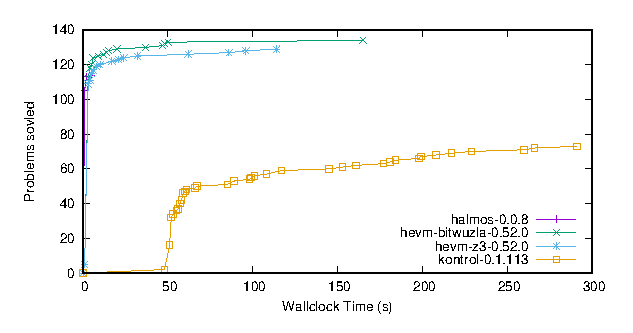
\includegraphics{cdf}
% \end{center}
% }

% [1] \qrcode[height=0.7cm]{https://github.com/eth-sc-comp/benchmarks/}\qquad  \url{https://github.com/eth-sc-comp/benchmarks/}
% \end{frame}

\begin{frame}[fragile=singleslide]{Limitations \& Future Work}
hevm has a number of inherent limitations:

\begin{itemize}
\item Loops are challenging. We have an iteration limit until which loops are examined
\item Recursion, and parametric calls can cause hevm to only partially explore the state
\item Complicated mathematical expressions (e.g. division, modulo) can cause a challenge
\item hevm is not verified, and neither are SMT solvers
\end{itemize}
\vspace{2ex}

Future work:
\begin{itemize}
\item Symbolic CopySlice handling
\item Better handling of loops and recursion: include into IR, and solve for invariant via CHC
\end{itemize}
\end{frame}

\begin{frame}[fragile=singleslide]{Quick Start Guide}
Development environment:
\begin{Verbatim}[frame=single, framerule=0.2mm, framesep=2mm,fontsize=\footnotesize]
sh <(curl -L https://nixos.org/nix/install) --daemon
git clone https://github.com/ethereum/hevm/
cd hevm
nix-shell
\end{Verbatim}

You now have in the shell:
\begin{itemize}
    \item hevm via cabal: \texttt{cabal run exe:hevm -- test/symbolic/equivalance}
    \item SMT solvers: Z3, bitwuzla, cvc5
    \item Ethereum development environment: solc, geth, evm, forge
\end{itemize}
\bigskip

\begin{Verbatim}[frame=single, framerule=0.2mm, framesep=2mm,fontsize=\footnotesize]
cabal run exe:hevm -- symbolic --create --code "60806040523480..."
\end{Verbatim}
\end{frame}

\begin{frame}{Thank you for your time!}
    Any questions?
\end{frame}

\end{document}
